\begin{exercise}
      {ID-24498813eb4bb3b16664c88043eab1a482632047}
      {Mario und Luigi}
  \ifproblem\problem\par
    Mario und Luigi sind mit dem Auto unterwegs. Sie wechseln sich beim
    Fahren ab. Wenn Luigi am Steuer sitzt, fahren sie doppelt so schnell wie
    mit Mario am Steuer. Auf der Fahrt von Adorf nach Bedorf fährt jeder die
    Hälfte der Zeit. Auf dem Rückweg nehmen sie dieselbe Strecke, allerdings
    fährt diesmal jeder die Hälfte des Weges. Für die Rückfahrt brauchen sie
    genau eine Stunde länger als für die Hinfahrt. Wie lange dauert die
    Hinfahrt?
  \fi
  \ifoutline\outline\par
    \begin{minipage}{0.49\textwidth}
      \centering
      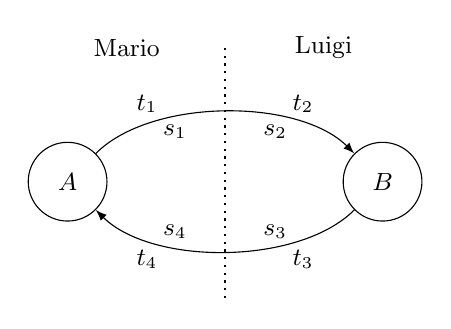
\begin{tikzpicture}
        \node[circle, minimum size=1cm, draw=black] (A) at (0, 0) {{\small$A$}};
        \node[circle, minimum size=1cm, draw=black] (B) at (4, 0) {{\small$B$}};
        \draw[->, >=latex] (A.45)  .. controls +( 45:1cm) and +(135:1cm) .. (B.135);
        \draw[->, >=latex] (B.225) .. controls +(225:1cm) and +(315:1cm) .. (A.315);
        \draw[style=dotted, line width=0.8pt] (2, 17mm) -- (2, -15mm);
        \node at (0.75, 17mm) {{\small Mario}};
        \node at (3.25, 17mm) {{\small Luigi}};
        \node[shift=(135: 9mm)] at (2, 0) {{\small$s_{1}$}};
        \node[shift=(135:14mm)] at (2, 0) {{\small$t_{1}$}};
        \node[shift=( 45: 9mm)] at (2, 0) {{\small$s_{2}$}};
        \node[shift=( 45:14mm)] at (2, 0) {{\small$t_{2}$}};
        \node[shift=(315: 9mm)] at (2, 0) {{\small$s_{3}$}};
        \node[shift=(315:14mm)] at (2, 0) {{\small$t_{3}$}};
        \node[shift=(225: 9mm)] at (2, 0) {{\small$s_{4}$}};
        \node[shift=(225:14mm)] at (2, 0) {{\small$t_{4}$}};
      \end{tikzpicture}
    \end{minipage}%
    \hfill
    \begin{minipage}{0.49\textwidth}
      \begin{equation*}
        \begin{split}
        v_{L}&=2\cdot v_{M} \\
        t_{1}=t_{2}&=\frac{t_{AB}}{2} \\
        s_{1}+s_{2}&=s_{3}+s_{4} \\
        s_{3}=s_{4}&=\frac{d}{2} \\
        t_{B\!A}&=t_{AB}+1
        \end{split}
      \end{equation*}
    \end{minipage}\bigskip
  \fi
  \ifoutcome\outcome\par
    \begin{minipage}{0.49\textwidth}
      \centering
      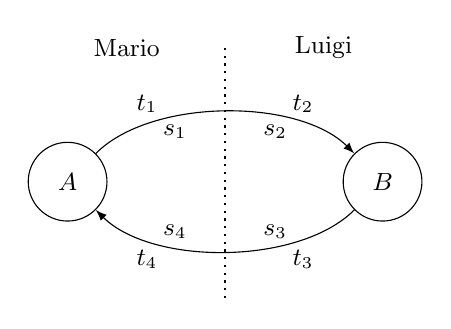
\begin{tikzpicture}
        \node[circle, minimum size=1cm, draw=black] (A) at (0, 0) {{\small$A$}};
        \node[circle, minimum size=1cm, draw=black] (B) at (4, 0) {{\small$B$}};
        \draw[->, >=latex] (A.45)  .. controls +( 45:1cm) and +(135:1cm) .. (B.135);
        \draw[->, >=latex] (B.225) .. controls +(225:1cm) and +(315:1cm) .. (A.315);
        \draw[style=dotted, line width=0.8pt] (2, 17mm) -- (2, -15mm);
        \node at (0.75, 17mm) {{\small Mario}};
        \node at (3.25, 17mm) {{\small Luigi}};
        \node[shift=(135: 9mm)] at (2, 0) {{\small$s_{1}$}};
        \node[shift=(135:14mm)] at (2, 0) {{\small$t_{1}$}};
        \node[shift=( 45: 9mm)] at (2, 0) {{\small$s_{2}$}};
        \node[shift=( 45:14mm)] at (2, 0) {{\small$t_{2}$}};
        \node[shift=(315: 9mm)] at (2, 0) {{\small$s_{3}$}};
        \node[shift=(315:14mm)] at (2, 0) {{\small$t_{3}$}};
        \node[shift=(225: 9mm)] at (2, 0) {{\small$s_{4}$}};
        \node[shift=(225:14mm)] at (2, 0) {{\small$t_{4}$}};
      \end{tikzpicture}
    \end{minipage}%
    \hfill
    \begin{minipage}{0.49\textwidth}
      \begin{equation*}
        \begin{split}
        v_{L}&=2\cdot v_{M} \\
        t_{1}=t_{2}&=\frac{t_{AB}}{2} \\
        s_{1}+s_{2}&=s_{3}+s_{4} \\
        s_{3}=s_{4}&=\frac{d}{2} \\
        t_{B\!A}&=t_{AB}+1
        \end{split}
      \end{equation*}
    \end{minipage}\bigskip

    Da der Hinweg genauso lang ist wie der Rückweg, gilt:
    \begin{alignat*}{2}
                 &       & s_{1}+s_{2}&=s_{3}+s_{4}                                               \\[2ex]
      \Rightarrow&\qquad & v_{M}\cdot t_{1}+v_{L}\cdot t_{2}&=v_{L}\cdot t_{3}+v_{M}\cdot t_{4}   \\[2ex]
      \Rightarrow&\qquad & \left(v_{M}+v_{L}\right)\cdot\frac{t_{AB}}{2}&=2\cdot v_{L}\cdot t_{3} \\[2ex]
      \Rightarrow&\qquad & 3\cdot v_{M}\cdot\frac{t_{AB}}{2}&=4\cdot v_{M}\cdot t_{3}             \\[2ex]
      \Rightarrow&\qquad & \frac{3}{2}\cdot t_{AB}&=4\cdot t_{3}
    \end{alignat*}
    Mit $t_{3}$ ist die Zeit gemeint, die Luigi auf dem Rückweg am Steuer sitzt:
    \begin{equation*}
      \begin{split}
        t_{3}&=\frac{s_{3}}{v_{L}}=\frac{d}{2v_{L}}=\frac{d}{4v_{M}}
        \qquad\qquad
        t_{4}=\frac{s_{4}}{v_{M}}=\frac{d}{2v_{M}}=2\cdot t_{3}\\[3ex]
        t_{B\!A}&=t_{3}+t_{4}=3\cdot t_{3}
        \quad\Rightarrow\quad
        t_{3}=\frac{1}{3}\cdot t_{B\!A}
      \end{split}
    \end{equation*}

    Zusammen gilt also:
    \begin{equation*}
      \frac{3}{2}\cdot t_{AB}=\frac{4}{3}\cdot t_{B\!A}
      \quad\Rightarrow\quad
      t_{AB}=\frac{8}{9}\cdot t_{B\!A}
    \end{equation*}

    Für $t_{AB}$ und $t_{B\!A}$ ergibt sich also folgendes lineares Gleichungssystem:
    \begin{equation*}
      \left|
      \begin{array}{lcl}
        t_{B\!A} & = & t_{AB}+1 \\
        t_{AB}   & = & \frac{8}{9}\cdot t_{B\!A}
      \end{array}
      \right.
    \end{equation*}

    Mit der Lösung:
    \begin{alignat*}{2}
                 &       &        t_{AB}&=\frac{8}{9}\cdot\left(t_{AB}+1\right) \\[2ex]
      \Rightarrow&\qquad & 9\cdot t_{AB}&=8\cdot t_{AB}+8                       \\[2ex]
      \Rightarrow&\qquad &        t_{AB}&=8
    \end{alignat*}

    Die Hinfahrt dauert also genau 8 Stunden.
  \fi
\end{exercise}
